\subsection{Algebraic definition of the cross product}

From its geometric description, we can prove that the cross product
satisfies the following properties.

\begin{proposition}{Properties of the cross product}{properties-cross-product}
  Let $\vect{u}, \vect{v}, \vect{w}$ be vectors in $\R^3$, and $k$ a
  scalar. Then the following hold.%
  \index{properties of cross product}%
  \index{cross product!properties}%
  \index{vector!cross product!properties}%
  \index{vector!properties of cross product}%
  \begin{enumerate}
  \item
    $\vect{u}\times \vect{v}= -(\vect{v}\times \vect{u})$,
    and $\vect{u}\times \vect{u}=\vect{0}$.
  \item $(k \vect{u})\times \vect{v}= k (\vect{u}\times \vect{v})
    =\vect{u}\times (k \vect{v})$.
  \item $\vect{u}\times (\vect{v}+\vect{w}) =\vect{u}\times \vect{v}+\vect{u}\times \vect{w}$.
  \item $(\vect{v}+\vect{w}) \times \vect{u}=\vect{v} \times \vect{u}+\vect{w}\times \vect{u}$.
  \end{enumerate}
\end{proposition}

\begin{proof}
  Formula $1$. follows immediately from the definition. The vectors
  $\vect{u}\times \vect{v}$ and $\vect{v}\times \vect{u}$ have the
  same magnitude, $\norm{\vect{u}}\norm{\vect{v}}\sin \theta$, and an
  application of the right hand rule shows they have opposite
  direction.

  Formula $2$. is proven as follows. If $k $ is a non-negative scalar,
  the direction of $(k \vect{u}) \times \vect{v}$ is the same as
  the direction of
  $\vect{u}\times \vect{v}, k (\vect{u}\times \vect{v}) $ and
  $\vect{u}\times (k \vect{v})$. The magnitude is $k$ times the
  magnitude of $\vect{u}\times \vect{v}$ which is the same as the
  magnitude of $k (\vect{u}\times \vect{v}) $ and
  $\vect{u}\times (k \vect{v})$. Using this yields equality in
  $2$. In the case where $k <0$, everything works the same way except
  the vectors are all pointing in the opposite direction and you must
  multiply by $\abs{k }$ when comparing their magnitudes.

  The distributive laws, $3$. and $4$., are harder to establish. For
  now, we will content ourselves with noticing that if we know that
  $3$. is true, $4$. follows. Namely, assuming $3$., and using $1$.,
  we have
  \begin{align*}
    (\vect{v}+\vect{w}) \times \vect{u}
    & =-\vect{u}\times (
      \vect{v}+\vect{w}) \\
    & =-(\vect{u}\times \vect{v}+\vect{u}\times \vect{w}) \\
    & =\vect{v}\times \vect{u}+\vect{w}\times \vect{u}.
  \end{align*}
\end{proof}

In turn, we can use the properties from
Proposition~\ref{prop:properties-cross-product} to get an algebraic
description of the cross product. We begin by determining the cross
products of the special vectors $\vect{i}$, $\vect{j}$, and
$\vect{k}$. They are as follows:
\begin{equation*}
  \begin{array}{c@{\quad\quad}c@{\quad\quad}c}
    \vect{i}\times \vect{j}=\vect{k},
    & \vect{j}\times \vect{i}=-\vect{k},
    & \vect{i}\times \vect{i}=\vect{0}, \\
    \vect{k}\times \vect{i}=\vect{j},
    & \vect{i}\times \vect{k}=-\vect{j},
    & \vect{j}\times \vect{j}=\vect{0}, \\
    \vect{j}\times \vect{k}=\vect{i},
    & \vect{k}\times \vect{j}=-\vect{i},
    & \vect{k}\times \vect{k}=\vect{0}.
  \end{array}
\end{equation*}
With this information and the laws of
Proposition~\ref{prop:properties-cross-product}, we can compute the
cross product of any two vectors from their coordinates.%
\index{cross product!coordinate description} Let
\begin{equation*}
  \vect{u}=\begin{mymatrix}{c}u_1\\u_2\\u_3\end{mymatrix}
  \quad\mbox{and}\quad
  \vect{v}=\begin{mymatrix}{c}v_1\\v_2\\v_3\end{mymatrix}.
\end{equation*}
Then we have:
\begin{eqnarray*}
  \vect{u}\times\vect{v}
  &=& (u_1\vect{i}+u_2\vect{j}+u_3\vect{k})\times (v_1\vect{i}+v_2\vect{j}+v_3\vect{k}) \\
  &=& \begin{array}[t]{@{}c@{~}c@{~}c@{~}c@{~}c@{~}c}
        & u_1v_1(\vect{i}\times\vect{i})
        &+& u_1v_2(\vect{i}\times\vect{j})
        &+& u_1v_3(\vect{i}\times\vect{k}) \\
        +& u_2v_1(\vect{j}\times\vect{i})
        &+& u_2v_2(\vect{j}\times\vect{j})
        &+& u_2v_3(\vect{j}\times\vect{k}) \\
        +& u_3v_1(\vect{k}\times\vect{i})
        &+& u_3v_2(\vect{k}\times\vect{j})
        &+& u_3v_3(\vect{k}\times\vect{k})
      \end{array}
  \\
  &=&\begin{array}[t]{@{}c@{~}c@{~}c@{~}c@{~}c@{~}c}
       & u_1v_1\vect{0}
       &+& u_1v_2\vect{k}
       &-& u_1v_3\vect{j} \\
       -& u_2v_1\vect{k}
       &+& u_2v_2\vect{0}
       &+& u_2v_3\vect{i} \\
       +& u_3v_1\vect{j}
       &-& u_3v_2\vect{i}
       &+& u_3v_3\vect{0}
     \end{array}
  \\
  &=& (u_2v_3-u_3v_2) \vect{i}+
      (u_3v_1 - u_1v_3) \vect{j}+
      (u_1v_2-u_2v_1) \vect{k}.
\end{eqnarray*}
The resulting formula for the cross product is summarized in the
following Proposition.

\begin{proposition}{Coordinate description of cross product}{cross-product-coordinate}
  The cross product can be computed as follows:
  \begin{equation*}
    \begin{mymatrix}{c}u_1\\u_2\\u_3\end{mymatrix}
    \times
    \begin{mymatrix}{c}v_1\\v_2\\v_3\end{mymatrix}
    =
    \begin{mymatrix}{c}
      u_2v_3 - u_3v_2 \\
      u_3v_1 - u_1v_3 \\
      u_1v_2 - u_2v_1 \\
    \end{mymatrix}.
  \end{equation*}
\end{proposition}

\begin{comment}
  There is another version of {\eqref{crossprod1}} which may be easier to remember.
  We can express the cross product as the determinant of a matrix, as follows.
  \begin{equation}
    \vect{u}\times \vect{v} = \begin{absmatrix}{ccc}
      \vect{i} & \vect{j} & \vect{k} \\
      u_1 & u_2 & u_3 \\
      v_1 & v_2 & v_3
    \end{absmatrix} \label{cross-prod3}
  \end{equation}
  Expanding the determinant along the top row yields
  \begin{equation*}
    \vect{i}(-1)^{1+1}\begin{absmatrix}{cc}
      u_2 & u_3 \\
      v_2 & v_3
    \end{absmatrix}+\vect{j}(-1)^{2+1}\begin{absmatrix}{cc}
      u_1 & u_3 \\
      v_1 & v_3
    \end{absmatrix}+\vect{k}(-1)^{3+1}\begin{absmatrix}{cc}
      u_1 & u_2 \\
      v_1 & v_2
    \end{absmatrix}\end{equation*}
  \begin{equation*}
    =\vect{i}\begin{absmatrix}{cc}
      u_2 & u_3 \\
      v_2 & v_3
    \end{absmatrix}-\vect{j}\begin{absmatrix}{cc}
      u_1 & u_3 \\
      v_1 & v_3
    \end{absmatrix}+\vect{k}\begin{absmatrix}{cc}
      u_1 & u_2 \\
      v_1 & v_2
    \end{absmatrix}\end{equation*}
  Expanding these determinants leads to
  \begin{equation*}
    (u_2v_3-u_3v_2) \vect{i}-(
    u_1v_3-u_3v_1) \vect{j}+(u_1v_2-u_2v_1)
    \vect{k}
    % \label{cross-prod4}
  \end{equation*}
  which is the same as {\eqref{crossprod2}}.
\end{comment}

We will now look at an example of how to compute a cross product.

\begin{example}{Find a cross product}{find-cross-product}
  Find $\vect{u} \times \vect{v}$ for the vectors
  \begin{equation*}
    \vect{u}
    =
    \begin{mymatrix}{r}
      1 \\
      -1 \\
      2
    \end{mymatrix}
    \quad\mbox{and}\quad
    \vect{v}
    =
    \begin{mymatrix}{r}
      3 \\
      -2 \\
      1
    \end{mymatrix}.
  \end{equation*}
\end{example}

\begin{solution}
  Using Proposition~\ref{prop:cross-product-coordinate}, we compute
  \begin{equation*}
    \begin{mymatrix}{c}1\\-1\\2\end{mymatrix}
    \times
    \begin{mymatrix}{c}3\\-2\\1\end{mymatrix}
    =
    \begin{mymatrix}{c}
      (-1)(1) - (2)(-2) \\
      (2)(3) - (1)(1) \\
      (1)(-2) - (-1)(3) \\
    \end{mymatrix}
    =
    \begin{mymatrix}{c}
      3 \\
      5 \\
      1
    \end{mymatrix}.
  \end{equation*}
\end{solution}

We use this concept in the following example.

\begin{example}{Area of a parallelogram}{area-parallelogram}
  Find the area of the parallelogram determined by the following
  vectors $\vect{u}$ and $\vect{v}$:
  \begin{equation*}
    \vect{u}
    =
    \begin{mymatrix}{r}
      1 \\
      -1 \\
      2
    \end{mymatrix}, \quad
    \vect{v}
    =
    \begin{mymatrix}{r}
      3 \\
      -2 \\
      1
    \end{mymatrix}.
  \end{equation*}
\end{example}

\begin{solution}
  Notice that these vectors are the same as the ones given in Example~\ref{exa:find-cross-product}.  Recall from the geometric description
  of the cross product that the area of the parallelogram is the
  magnitude of $\vect{u} \times \vect{v}$.  From
  Example~\ref{exa:find-cross-product},
  $\vect{u} \times \vect{v} = \mat{3,5,1}^T$.
  Thus the area of the parallelogram is
  \begin{equation*}
    \norm{\vect{u} \times \vect{v}} =
    \sqrt{3^2+5^2+1^2} = \sqrt{35}.
  \end{equation*}
\end{solution}

We can also use this concept to find the area of a triangle, as in the
following example.

\begin{example}{Area of triangle}{area-triangle}
  \index{cross product!area of triangle}%
  \index{area!of triangle}%
  \index{triangle!area of}%
  Find the area of the triangle determined by the points
  $(1,2,3)$, $(0,2,5)$, and $(5,1,2)$.
\end{example}

\begin{solution}
  Let $P=(1,2,3)$, $Q=(0,2,5)$, and $R=(5,1,2)$. The area
  of the triangle is exactly half of the area of the parallelogram
  determined by the vectors $\longvect{PQ}$ and $\longvect{PR}$.
  \begin{center}
    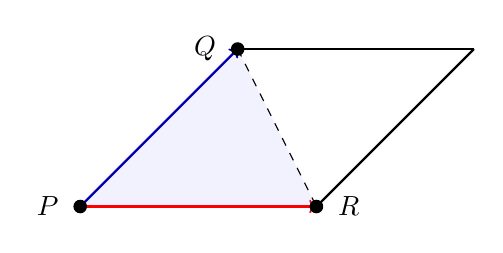
\begin{tikzpicture}[scale=1]
      \fill[blue!5] (0,0) -- (2,2) -- (3,0) -- cycle;
      \draw[->,thick,blue!70!black] (0,0) -- (2,2);
      \draw[->,thick,red] (0,0) -- (3,0);
      \draw[thick] (2,2)--(5,2);
      \draw[thick] (3,0)--(5,2);
      \draw[dashed] (2,2)--(3,0);
      \draw[fill](0,0) circle [radius=2.25pt] node[left=1ex]{$P$};
      \draw[fill](2,2) circle [radius=2.25pt] node[left=1ex]{$Q$};
      \draw[fill](3,0) circle [radius=2.25pt] node[right=1ex]{$R$};
    \end{tikzpicture}
  \end{center}
  We have $\longvect{PQ}=\mat{-1,0,2}^T$ and
  $\longvect{PR}=\mat{4,-1,-1}^T$. The area of the parallelogram is
  the magnitude of the cross product:
  \begin{equation*}
    \norm{\longvect{PQ}\times\longvect{PR}}
    =
    \norm{\begin{mymatrix}{r}
        -1 \\
        0 \\
        2
      \end{mymatrix} \times \begin{mymatrix}{r}
        4 \\
        -1 \\
        -1
      \end{mymatrix}
    }
    = \norm{\begin{mymatrix}{rrr}
        2 \\ 7 \\ 1
      \end{mymatrix}
    }
    = \sqrt{2^2+7^2+1^2}
    = \sqrt{54}.
  \end{equation*}
  Hence the area of the triangle is $\frac{1}{2}\sqrt{54}= \frac{3}{2}\sqrt{6}$.
\end{solution}

In general, the area of the triangle determined by three points
$P,Q,R$ in $\R^3$ is given by
\begin{equation*}
  \frac{1}{2}\norm{\longvect{PQ} \times  \longvect{PR}}.
\end{equation*}
